\section{Discussion}
\label{s:discussion}

\subsection{Effect of Penalty Parameter}
\label{s:discussion_pp}

\paragraph{}Equation (\ref{1.6}) in which residuals are measured with $\ell_2$ norm and regularization is 
done with $\ell_1$ norm, seeks the solution that is close (in $\ell_2$ norm) to the 
measured corrupted signal $b$ and the one that is sparse. By varying the penalty parameter $\lambda$
( aka regularization parameter) one can find out the optimal trade-off between $\parallel Ax-b \parallel_{\ell_2}$
(fidelity term)and $\parallel x \parallel_{\ell_1}$( sparsity inducing term ).
\paragraph{}Penalty parameter varies form 0 to $\infty$. In practical applications, for smaller value of $\lambda$ in 
 equation (\ref{1.6}) put more emphasis on fidelity term, thereby neglecting sparsity in the solution. On the other
hand, larger values of $ \lambda$ put more weight on sparsity inducing term and leads to
sparsest solution which is zero vector. So finding out the optimal trade-off between these bi-criterion objectives requires
optimal value of regularization parameter.
\paragraph{}Figure \ref{Figsmalllam} shows the reconstructed image of single point source with point source 
at the center. Due to very small $\lambda=10^{-4}$, this leads to just the least solution which is not sparse.
\paragraph{}Figure \ref{Figlargelam} shows the reconstructed image of same single point source with point source 
at the center. Large value $\lambda=10^{4}$ gives zero solution as discussed.
\paragraph{}For certain optimal $\lambda = 1150$ (found out by simulations), Figure  shows reconstruction
of single point source exactly.

\begin{figure}[!htbp]
  \begin{center}
      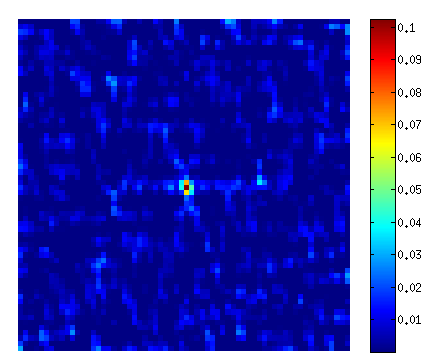
\includegraphics[width=4in,height=3in]{figures/spsn}
    \caption{Reconstruction of single point source for $\lambda = 0.001$}
    \label{Figsmalllam}
  \end{center}
\end{figure}

\begin{figure}[!htbp]
  \begin{center}
      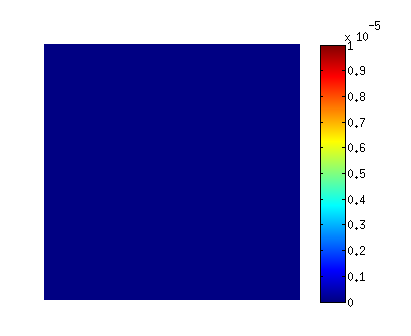
\includegraphics[width=5in,height=4in]{figures/spss}
    \caption{Reconstruction of single point source  for $\lambda = 10000$}
    \label{Figlargelam}
  \end{center}
\end{figure}

\newpage
\subsection{Convergence of algorithms}
\label{s:discussion_convergence}

\begin{figure}[!htbp]
  \begin{center}
      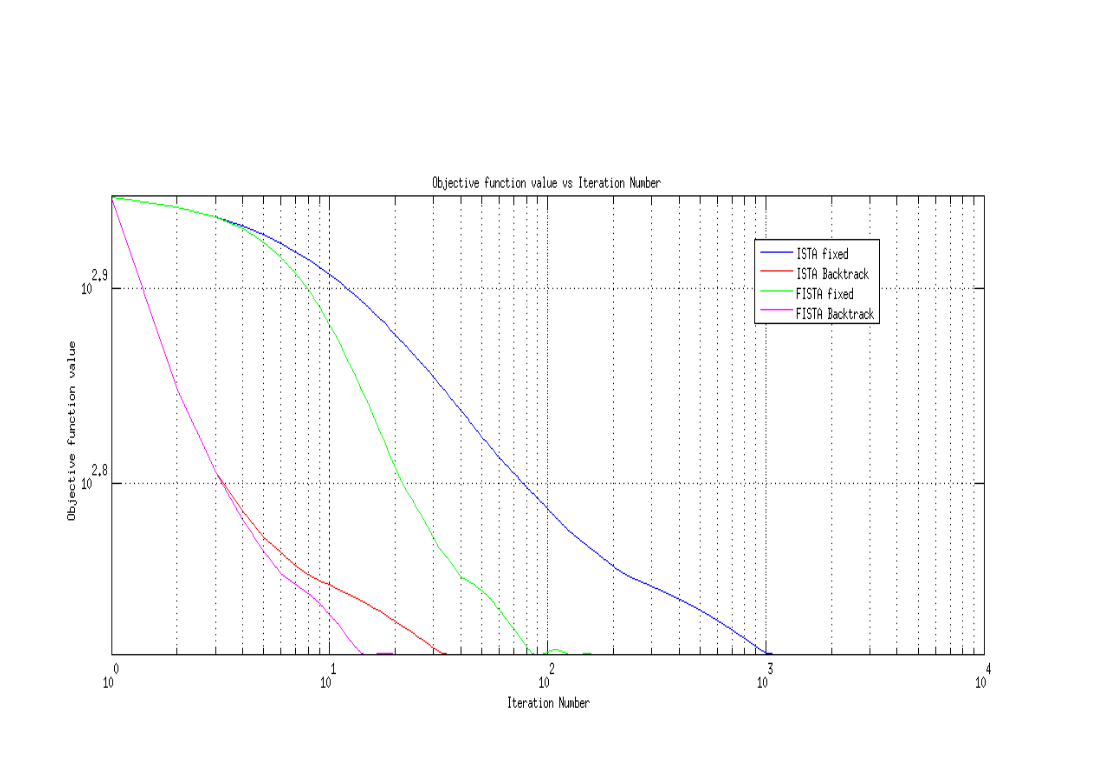
\includegraphics[width=6.1in,height=4in]{figures/convergence}
    \caption{Convergence of Algorithms}
    \label{Figconvergence}
  \end{center}
\end{figure}

\paragraph{}Figure \ref{Figconvergence}, shows the convergence of algorithms with 
respect to iteration number. It is clear that FISTA shows better performance 
than ISTA algorithms which is also theoretically proved. Further backtracking variants of both algorithms seems to 
perform much better then their corresponding fixed step size variants. All
four algorithms reaches the same optimal value and with same reconstructed image.

\newpage
\subsection{Flux fidelity}
\label{s:discussion_ff}

\paragraph{}Single point source and double point source reconstruction discussed in last chapter
are done with varying fluxes of illuminated pixels of image. This is done to check flux fidelity
with the penalty parameter. We have used various data set for single point source of fluxes 0.05, 0.1,
0.5, 1, 10 and 100 and double point sources we have used flux ratios as 0.1, 0.2, 0.4, 0.6 and 0.8.
\ref{Figflux} shows one of the result for single point source of flux 0.4.

\paragraph{}Figure \ref{Figflux} shows the plot peak value of the reconstructed image of 
single point source with flux value 0.4 (discussed in Section 6.3) with respect to penalty parameter varying from $10^-4$
to $10^4$ (Reconstructed Images in this range of penalty parameter can be seen in Fig 6.3 in 
Chapter 6). It is clear from the plot that certain optimal range of penalty parameter flux of 
single point source recovered is 0.4. 


\begin{figure}[!htbp]
  \begin{center}
      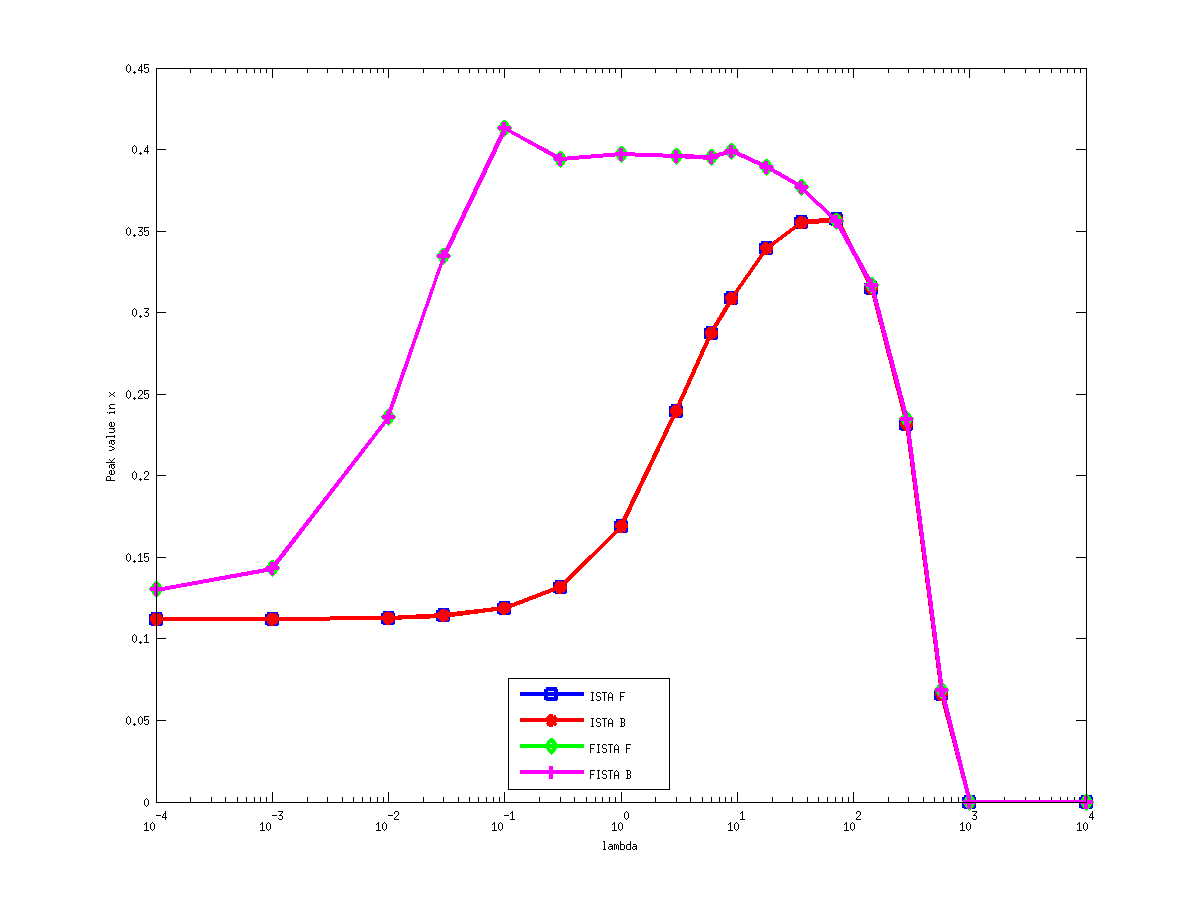
\includegraphics[width=6.1in,height=4in]{figures/pv}
    \caption{Peak Value vs Penalty Parameter}
    \label{Figflux}
  \end{center}
\end{figure}
